Despite some limitations, there are some strong positive outcomes from this study. The methodological framework designed for the thesis manages to combine two seemingly dis-aligned approaches to futures studies: forecasting (in the form of CLDs) and backcasting. While there are articles in the literature of similar efforts, such as \textcite{kok2011_Combiningparticipativebackcasting} and \textcite{dortmans2005_Forecastingbackcastingmigration}, the difference lies in the integration method used in this research: the Multi-Level Perspective on sustainable transitions. \fref{f:discussion-methodology} presents a conceptual visualisation of the integration role that transitions theory plays in the thesis. To understand the importance of the contribution of this study, the following paragraphs describe the drawbacks of adhering to a single approach for policy assessment (either forecasting or backcasting). It is argued that the use of the MLP overcomes those limitations, thus becoming a prominent ``result'' of this thesis.

\begin{figure}
\centering
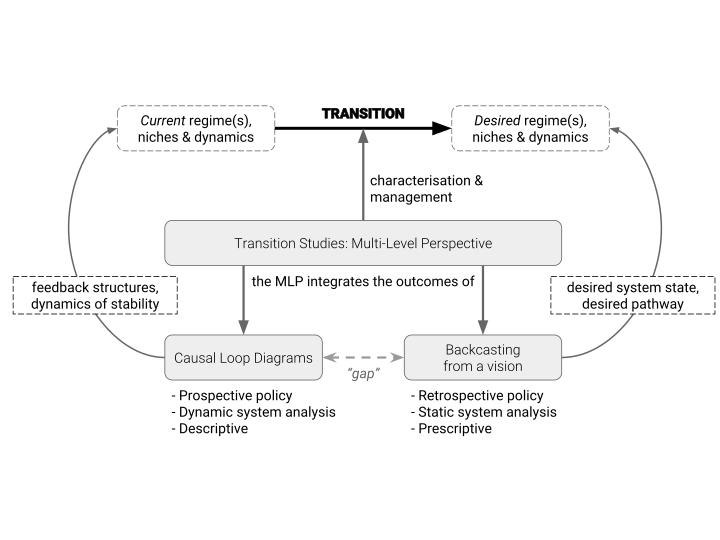
\includegraphics[clip,trim=0 3cm 0 3cm,width=\linewidth]{figures/discussion-methods.pdf}
\caption[Integrative power of transition theory]{Transition theory can bridge the gap between futures studies and forecasting tools, by translating the insights from each into the same language (discourse).}
\label{f:discussion-methodology}
\end{figure}

On one hand, forecasting tools (CLDs and System Dynamics, for example) are commonly used to inform policy makers of the possible development scenarios, but fail to convey normative insights: they are inherently \emph{descriptive} methods. Another weakness of using forecasts as the basis for policy making is that no space is available for radical innovation. This is, predictions based on present system structures cannot take into account structural change or unexpected developments. The policies that emerge from using forecasts are \emph{prospective}. On the other hand, the strength of forecasts and System Dynamics (CLDs) in particular, is the capability to analyse \emph{dynamic}\footnote{Again, the dynamism captured by these tools is constrained to the modelled structure of the system.} behaviours. Dynamics and feedback structures are very important to policy assessment, because they are sources of policy resistance mechanisms, such as rebound effects.

Backcasting and ``desirable'' visions methods are, on the contrary, normative in nature, this is, they are \emph{prescriptive} in their analysis (or discussion) of the systems under scope. However, unless explicitly incorporated in the processes, the perspective of the systems is rather \emph{static}. Even though they are used to convey the desired changes (dynamism over time), they do not account for feedback structures nor for dynamic system behaviour. In the context of sustainable transitions, a final feature of backcasting is appealing as a methodology: the \emph{retrospective} approach to policy design. The fact that backcasting processes start from a desired end-state opens the possibility to include radical innovation or, simply, ``radical'' changes that would be unthinkable from the present system condition.

The use of the MLP in the thesis as a discursive translation tool serves the purpose of overcoming the limitations described above, while benefiting from the strengths of each tool. (1) The focus on co-evolution and dynamism (stability and change) of socio-technical niches, regimes and landscapes fits perfectly the notion of system dynamics captured by CLDs. (2) While not normative per se, the MLP can still accommodate the results of a backcasted pathway to a normative future vision. (3) The context of a ``transition'' embeds desired future visions and pathways and, therefore, policy design can be made retrospectively, allowing broader possibilities to be included and for policies that support radical innovation. Finally, the multidisciplinary approach of the MLP supports an analysis scope broader than that of the formal models of System Dynamics, similarly to backcasting.

As the concluding remark, the aforementioned use of the MLP approach is, as argued, a significant contribution to sustainability research. It could, to some extent, be regarded as a form of \emph{transition management} \parencite{rotmans2001_Moreevolutionthan,kemp2011_TransitionManagementas}, although it differs in some aspects: different emphasis on culture, inclusion of subaltern combined methodologies and, following the transitions governance scheme described by \textcite{kemp2007_Transitionmanagementas}, this thesis is situated only at a strategic management level. However, the approach taken can benefit other sustainability studies in the following situations:
\begin{enumeratealpha}
\item A (participatory) process has delivered a desirable vision and/or pathway to a sustainable future, but there are uncertainties with regards to required structural changes or policy resistance mechanisms.
\item A forecasting study has provided decision makers with a thorough understanding of the current system and its feedback mechanisms but, even at the light of possible scenarios described by the forecast, they are unsure of what normative actions should be taken.
\end{enumeratealpha}
In both cases, a complementary study can be performed and the results can be then harmonised using an MLP approach. This integration framework is, indeed, the most interesting outcome of the thesis.